\documentclass[lang=cn,zihao=-4,twoside,fontset=none]{textbook}
\usepackage{pdfpages}
\definecolor{gray50}{gray}{0.5}
\definecolor{Dblue}{RGB}{1,74,126}
\definecolor{Sblue}{RGB}{2,121,202}
\newcommand\dottedline[1][]{%
   \tikz[baseline]\draw[line width=3pt,dotted,line cap=round,dash pattern=on 0pt off 3\pgflinewidth, gray50](0,-1.2)--(0,1.8);
}
% ----------------------------- Math Font ------------------------------------- %
\usepackage{newtxmath}
\DeclareSymbolFont{CMlargesymbols}{OMX}{cmex}{m}{n}
\let\sum\relax
\let\prod\relax
\DeclareMathSymbol{\sum}{\mathop}{CMlargesymbols}{"50}
\DeclareMathSymbol{\prod}{\mathop}{CMlargesymbols}{"51}
%% \infty
\DeclareSymbolFont{symbolsCM}{OMS}{cmsy}{m}{n}
\SetSymbolFont{symbolsCM}{bold}{OMS}{cmsy}{b}{n}
\let\txinfty\infty
\DeclareMathSymbol{\infty}{\mathord}{symbolsCM}{"31}
\pagecolor{lightgray!10}
% ---------------------------------------------------------------------------- %
\begin{document}
%----------------------------------------------------------------------------------------
%	标题页信息
%----------------------------------------------------------------------------------------
\title{论文改进汇总}
\subtitle{工作指南与进度追踪}
\author{Ethan Lu}
\date{\zhtoday}
\publishers{自制}
%----------------------------------------------------------------------------------------

%----------------------------------------------------------------------------------------
%	插入自定义标题页
%----------------------------------------------------------------------------------------
\begin{titlepage} % 创建一个新的页面
    %用来将图片从左下角开始平铺整个封面
        \AddToShipoutPicture*{%
        \AtPageLowerLeft{%
            \adjustbox{width=1.1\paperwidth, height=1.5\paperheight, keepaspectratio}{% 强制图片至纸张尺寸,但可能裁切
                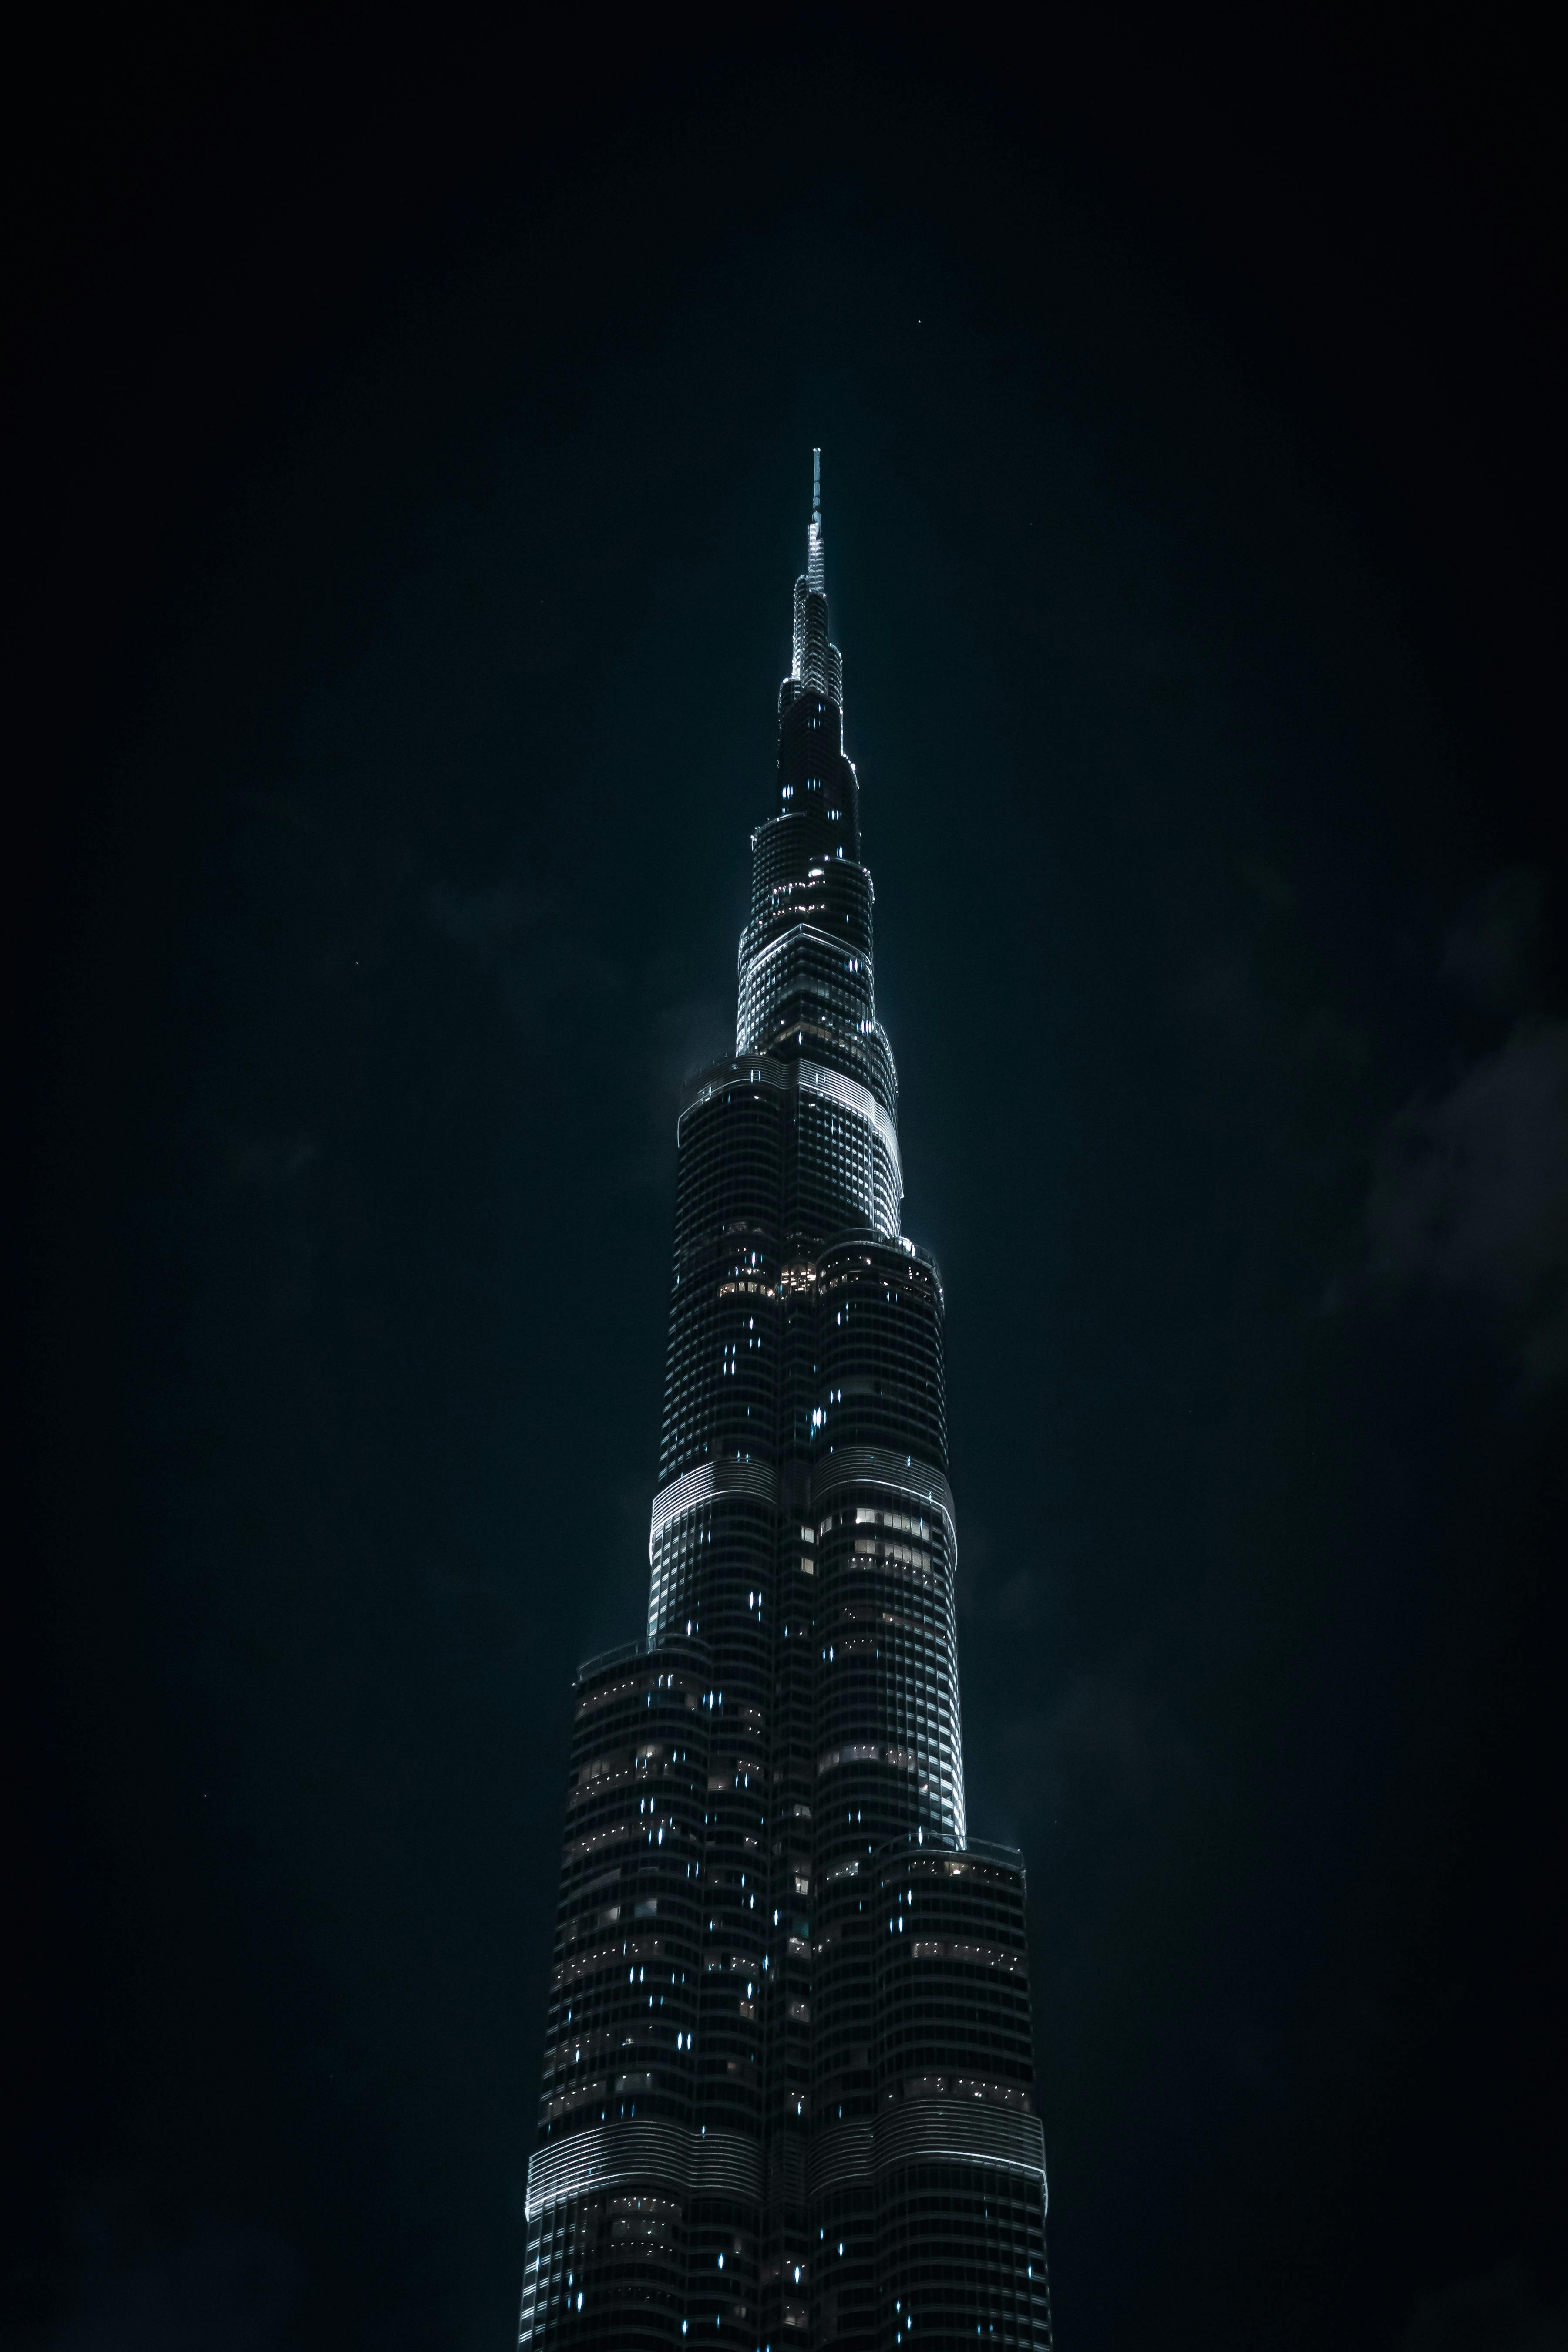
\includegraphics{images/pexels-photo-3378916.jpeg}
            }
        }
    }
    \begin{flushleft} % 左对齐环境
        \setlength{\leftskip}{1cm} % 左侧缩进
        \makeatletter % 允许访问带有@字符的内部命令
        % \vspace*{4cm} % 标题距离页面顶端的空白
        % {\color{white}\Huge \textbf{\@title} \par} % 使用前文定义的title作为标题
        % \vspace{1cm} % 标题和子标题的间距
        % {\color{white}\Large \@subtitle \par} % 使用前文定义的subtitle作为子标题
        % \vfill % 作者信息前的垂直填充
        % {\color{white}\large \@author \par} % 作者名
        % {\color{white}\large \@publishers \par} % 出版者
        % {\color{white}\large \today\par} % 日期,默认为当天
            \begin{tikzpicture}[overlay,remember picture]
            \begin{pgfonlayer}{bottom}
                \fill[dblue!10,opacity=0.1] (current page.south west) rectangle ++(\paperwidth,2cm);
                \node[inner sep=0pt,text=white,font=\large\sffamily,above] (bottominfo) at ([yshift=.7cm]current page.south) {
                    \@author\hspace{4cm}\@publishers\hspace{4cm}\today
                };
            \end{pgfonlayer}
            \fill[color=black!50,opacity=.2]node[append after command={
                ([yshift=0.5cm]bookinfo.north west) rectangle ([yshift=-0.5cm]bookinfo.south east)},minimum width=\paperwidth,opacity=1,align=left,inner sep=0pt,anchor=west] (bookinfo) at ([shift={(0,4cm)}]current page.west) {\hspace{-7cm}
                    \begin{varwidth}{\linewidth}
                        \setlength\baselineskip{3ex}
                        \textcolor{black!10!white}{\Huge \textbf{\@title}} \\[.6cm]
                        \textcolor{black!10!white}{\Large \@subtitle}
                    \end{varwidth}
                    };
        \end{tikzpicture}
        \makeatother % 将@重置为非字母字符
        \vspace{0cm} % 标题和子标题的间距
        % 结束左对齐环境
    \end{flushleft}
    \ClearShipoutPicture % 清除背景图片
    \end{titlepage}
% --------------------------------- 主要内容写在下面 --------------------------------- %
\pagestyle{Mainpage} % 页面样式
\chapimg{images/pexels-photo-1452701.jpeg}

\newgeometry{left=2cm,right=2cm,top=2.5cm,bottom=2.2cm}
\tableofcontents
\restoregeometry
% ---------------------------------------------------------------------------- %

\partimg{images/pexels-photo-931018.jpeg}
\part{论文的审稿意见与修改方针}

\chapter[关于第一篇论文的审稿意见与见解探讨]{关于``Logarithmic vanishing theorems on weakly 1-complete K\"ahler manifolds'' 的审稿意见与修改方针}

% ---------------------------------------------------------------------------- %
\section{审稿意见分析}
\sidenote[][1cm]{\shufang\footnotesize 这一页是翻译,下一页是原稿。} 本文在Huang,Liu,Wan和Yang的工作基础上,推广了弱1 -完备Kahler流形的对数消没定理,他们建立了紧致K\"ahler流形的类似结果。主定理保证了某些上同调群在特定条件下的消失性,从而将紧致集合中已有的结果推广到更广泛的弱1 -完备流形类。


虽然这种扩展在数学上是正确的,但其方法紧紧地遵循了Huang等人使用的分析技术,特别是他们的$L^2$ -方法和逼近定理的使用。事实上,\textbf{本文基本上将他们的论点应用到弱$1$ -完备的K\"ahler流形上,而没有遇到重大的新挑战或在所使用的技术上引入实质性的创新} \sidenote{对此,我并不完全赞同。首先,我的方法结合了HLWY与逼近定理,通过一致估计找到合适的逼近定理显然是有一定创新的,而且,这个估计定理最终需要通过结合HLWY发展的良层同构来从$Y_i$上转化为$X_i$上,这显然也是有着独特的思考在内,不能一味地否定我的独立思考成果,而将所有都归结于他人的方法与结果,这明显不合理!}。


从历史上看,消失定理在代数几何和复分析中都起到了至关重要的作用,最早可以追溯到经典的Akizuki -- 小平-- Nakano紧致K\"ahler流形上的消失定理,并得到了广泛的应用.这些结果推广到非紧和弱1 -完备情形,由Norimatsu、埃斯诺和菲韦格等研究者开创,延续了这一趋势。
这些推广旨在探索更广泛几何背景下的上同调行为,Huang等人的工作代表了将这些思想推广到紧致K\"ahler流形上的关键发展。

\softclearmargin
本文的作者试图通过从紧致K\"ahler流形到弱1 -完备K\"ahler流形来对这一正在进行的研究做出贡献。
\textit{然而,这种转变显得相对直截了当,并没有遇到显著的额外困难。构造合适的Hermitian度量和使用Poincar\'e型度量的核心障碍在紧致情形下与以前的结果大致相同\sidenote{说的如此容易,那为何到现在还没人做出这方面的考虑呢?虽然碍于作者本人的思考深度和广度以及所掌握的知识有限性,没有办法创造具有独创性的方法来达成证明,但是能够就已有之方法来通过巧妙的组合运用来证明新发现的定理,这本就是创新。而且,就我所知,这里构造恰当的完备Hermitian度量也很巧妙地运用了H\"ormander发展的$L^2$估计理论,将寻找完备的K\"ahler度量转化为构造合适的Poincar\'e 度量,这使得难度大大降低,虽然这个方法是HLWY首先找到的,但是这无法改变我所设置的独特的Poincr\'e 度量-这一创新的有效性。}。}  因此,虽然总体的贡献是正确的,但似乎缺乏新颖性和难度,这将不满足《微分几何及其应用》的典型预期。


总之,\textbf{尽管本文在技术上对现有结果进行了合理的扩展,但它并没有引入黄,刘,万和杨已经建立的新方法或见解} \sidenote{这个新方法和新见解在何处呢?有待求证!}。因此,\textit{我不确定这篇文章的贡献是否足以达到本刊的标准} \sidenote{不清楚这个期刊的标准是什么?如此高,匪夷所思????}。
\clearpage
% 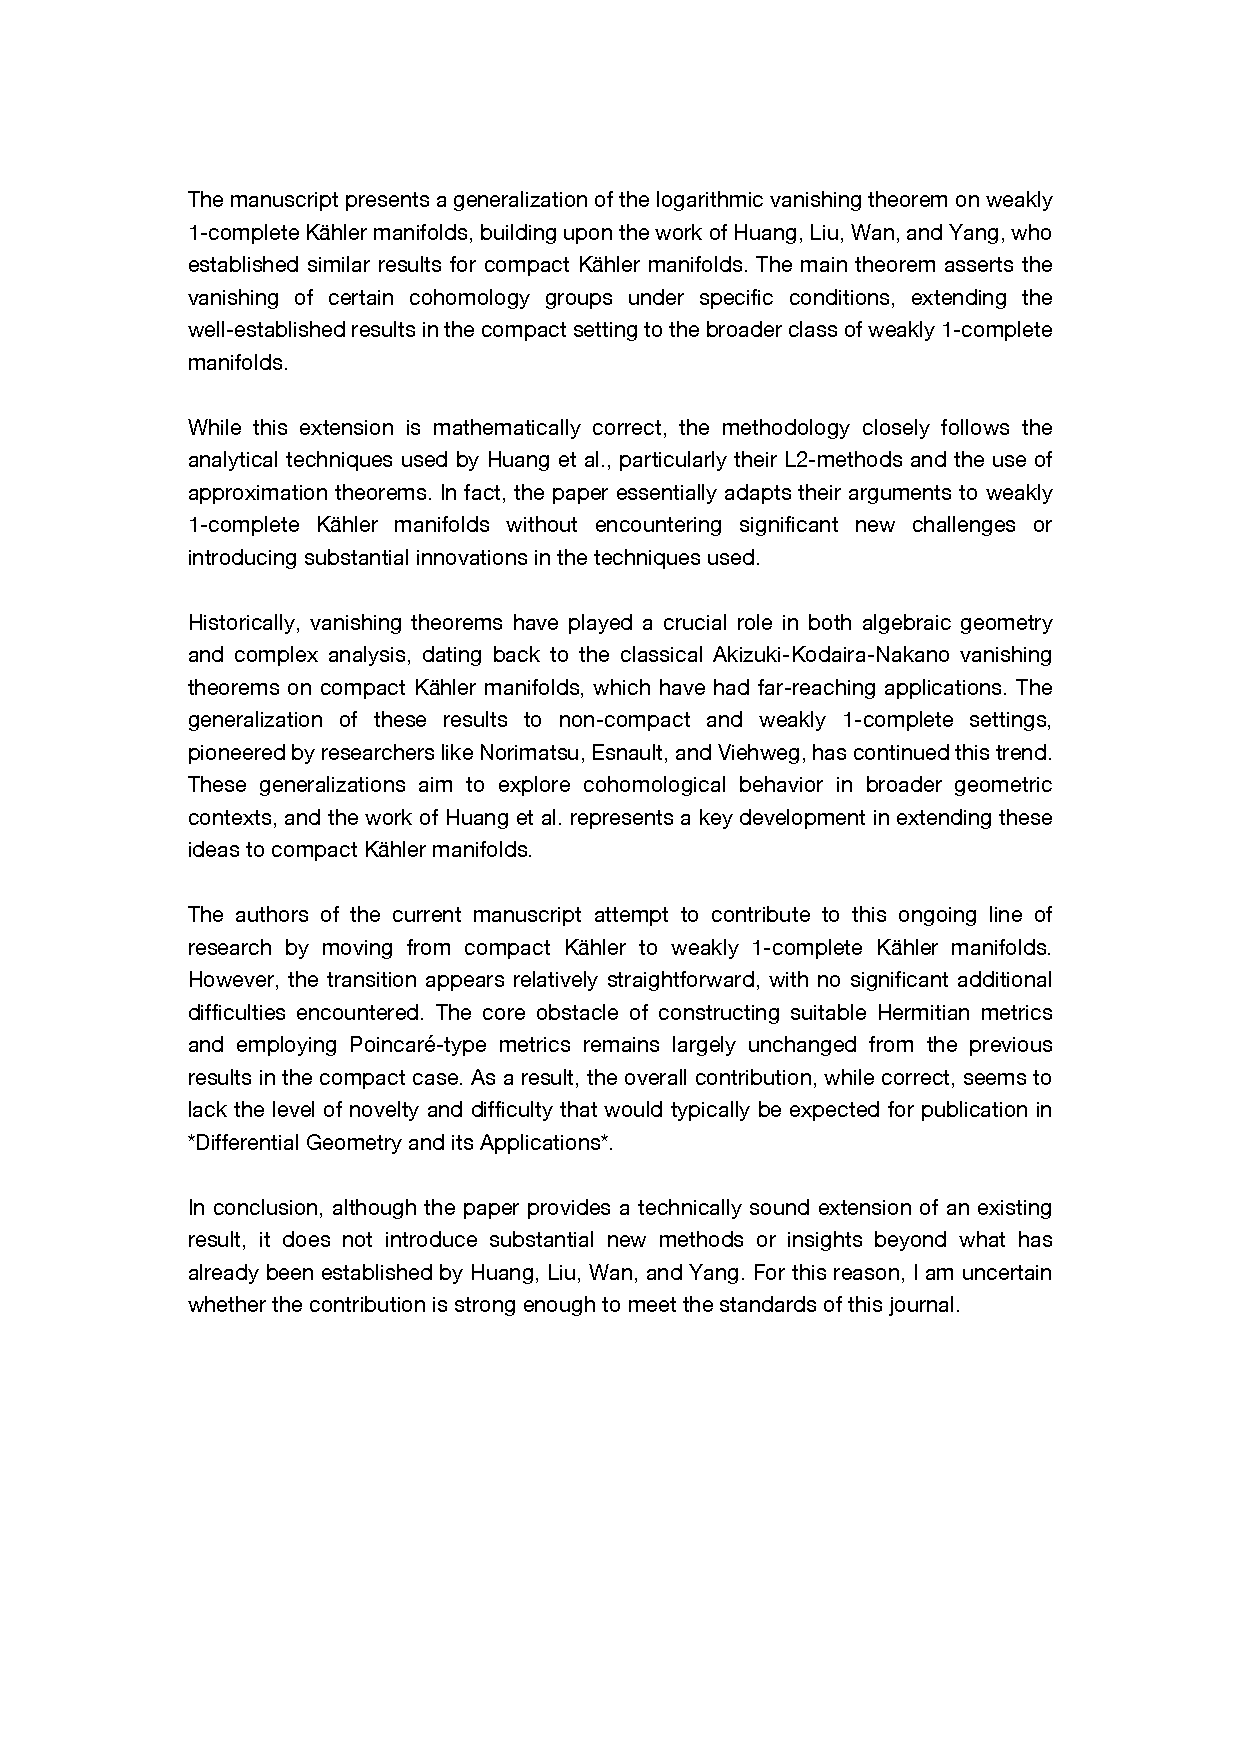
\includepdf[pages={1}]{images/review-log vanishing.pdf}% 注意filename提前准备好,一般放在同一路径下
\newpage
\section{修改方针}
\subsection{创新性}


\chapter[关于第二篇论文的审稿意见与见解探讨]{关于《\texorpdfstring{$L^q$}{L^q} extension theorem for jets on weakly pseudoconvex K\"ahler manifolds》的审稿意见与修改方针}

% ---------------------------------------------------------------------------- %
\section{审稿意见分析}
\begin{enumerate}
    \item \textbf{证明方法是否存在错误}

    在目前审阅的内容中,\textbf{数学上的证明}并没有明显的致命错误。然而,以下几点需要进一步注意:

    \begin{itemize}
        \item \textbf{精确性和细节推导}:文中的某些证明依赖于之前文献中的技术和结果,比如 \textbf{Demailly} 和 \textbf{Popovici} 的工作。然而,在某些关键步骤中,推导过于简略,特别是在复杂几何和全纯分析的背景下。虽然方法正确,但一些中间步骤未解释清楚。这种简化可能会让读者难以理解推导过程,甚至可能遗漏一些边界情况或特殊情形。

        \item \textbf{奇异性处理}:在弱伪凸Kähler流形上处理 jets 的扩展定理时,奇异性的处理方法较为复杂。如果论文在推导过程中对奇异性控制不严谨(比如度量奇点附近的估计不足),则可能导致最终结果不成立。这一点是需要特别检查的关键点。
    \end{itemize}

    \item \textbf{方法与参考文献过于相似的潜在问题}

    从你的描述中,该论文的主要结果是将参考文献中的方法推广到了 jets 的情形上。这里有几个需要注意的方面:

    \begin{itemize}
        \item \textbf{延续原有方法的合法性}:如果你将参考文献中的定理应用于新的上下文(例如 jets 的扩展),那么证明的每一步都必须严格验证适用于新的情形。这包括:推广过程中所用的假设是否在新的几何背景下成立,jets 的特殊性质是否带来新的困难或条件,是否需要针对 jets 的性质引入新的技巧。如果这些方面没有充分考虑,则可能存在方法上的缺陷。

        \item \textbf{新结果的独立性}:虽然使用已有的技术方法是学术研究中常见的做法,但为了避免与已有工作过于相似,你的工作必须在某些方面有实质性的创新或推广。如果只是简单地套用原有方法而没有足够的扩展或创新,那么在学术上可能被认为贡献有限。
    \end{itemize}

    \item \textbf{潜在的致命错误或漏洞}

    要判断是否存在致命错误可能使论文作废,我们需要重点关注以下几个方面:

    \begin{itemize}
        \item \textbf{基本假设的有效性}:在使用参考文献中的技术时,你是否重新检查了论文中的假设条件是否完全适用于 jets 情形?比如,在弱伪凸Kähler流形上的正则性条件、奇异度量的行为等,这些条件的有效性是整个证明体系的基础。如果基本假设不成立,整个证明将失效。

        \item \textbf{技术细节的稳健性}:对于复杂的全纯分析问题,技术细节(如估计、解析延拓等)通常非常脆弱。如果你在论文中使用了与参考文献相同的方法,但没有处理 jets 中新增的复杂性,这可能会导致错误。例如,jets 在扩展过程中的范数控制问题,可能与原文的情况不同,简单延续原有方法可能无法处理这些新的技术问题。

        \item \textbf{新情形下的定理适用性}:有时在推广某个定理时,新情形可能带来无法预见的障碍。如果你在证明过程中忽略了 jets 的特性(如更高阶微分的复杂性或几何结构的变化),可能导致证明结果不成立。
    \end{itemize}

    \item \textbf{结论}

    从目前的分析来看,\textbf{如果证明中的假设条件在推广过程中没有仔细检查,或者处理 jets 的特殊性时过于依赖原文的方法,而没有针对新问题作出调整},这可能会成为论文的主要问题。如果只是形式上将已知结果应用于 jets 上,而未能有效解决扩展过程中的技术难题,那么论文可能会面临学术上的批评。

    建议你重点检查以下几个问题:
    \begin{itemize}
        \item 证明的每一步是否严格适用于 jets 的情形?
        \item 所有使用的假设条件在新情形下是否依然成立?
        \item 是否有必要引入新的方法来处理 jets 的特殊性?
    \end{itemize}

    如果在这些方面没有漏洞,论文应该是可以成立的,但如果在处理这些问题时缺乏严谨性,可能会影响论文的有效性。
\end{enumerate}
\newpage
\section{修改方针}
\subsection{创新性}

\appendix
\part{原论文附件}
\chapter{论文原件}

% ---------------------------------------------------------------------------- %
\section{第一篇论文原稿}
\includepdf[pages={1-16}]{chapters/Logarithmic_theorems_on_weakly_1-complete_kahler_manifolds.pdf}% 注意filename提前准备好,一般放在同一路径下
\newpage
\section{第二篇论文原稿}
\includepdf[pages={1-14}]{chapters/L2extension_thoerem_of_jet.pdf}% 注意filename提前准备好,一般放在同一路径下
%
\printbibliography[heading=bibintoc]
 %
\end{document}


